\documentclass[11pt]{article}
\usepackage[a4paper,left=1in,right=1in,top=1in,bottom=1in]{geometry}

\usepackage[english]{babel}
\usepackage[T1]{fontenc}
\usepackage[utf8]{inputenc}
\usepackage{seqsplit}

\renewcommand{\familydefault}{\sfdefault}
\usepackage{setspace}  \singlespacing
\usepackage{graphicx}
\usepackage[absolute]{textpos}
\usepackage{xcolor}
\usepackage{fontawesome5}
\usepackage{multirow}
\usepackage{hyperref}
\usepackage{tcolorbox}
\hypersetup{
    colorlinks,
    linkcolor={red!50!black},
    citecolor={blue!50!black},
    urlcolor={blue}
}

\definecolor{mgray}{gray}{0.85}
\definecolor{mpurple}{HTML}{68236D}
\usepackage{float}
\usepackage{subfig,wrapfig}
\usepackage{amsmath,amsfonts,amsthm,amssymb}
\usepackage{fancyhdr,fancybox,color}
\usepackage{enumerate}
\usepackage[amssymb]{SIunits}
\definecolor{MyBlue}{rgb}{0,0.3,0.6}
\usepackage[all]{hypcap}
\usepackage{csquotes}
\usepackage[url=false,
backend=bibtex,
style=authoryear-comp,
doi=true,
isbn=true,
backref=false,
dashed=false,
maxcitenames=2,
maxbibnames=99,
natbib=true]{biblatex}
\DeclareNameAlias{author}{family-given}
\renewbibmacro{in:}{}
\addbibresource{../_logosAndRef/references.bib}
\nonfrenchspacing

\newlength{\headertobodysep}
\setlength{\headertobodysep}{1cm}

\begin{document}
\thispagestyle{empty}

\textblockorigin{0pt}{0pt}

\begin{textblock*}{5cm}(0.5cm,1cm)
    
\includegraphics[height=2cm]{../_logosAndRef/Durham-University.pdf}
\end{textblock*}

\begin{textblock*}{9cm}(6cm,1.5cm)
    \centering
    {\large \textbf{Coated Landau--Levich | CoMPhy Lab}}\\[0.2em]
    Department of Physics, Durham University\\[0.3em]
    \href{https://comphy-lab.org}{comphy-lab.org}
\end{textblock*}

\begin{textblock*}{5cm}(15.5cm,1cm)
    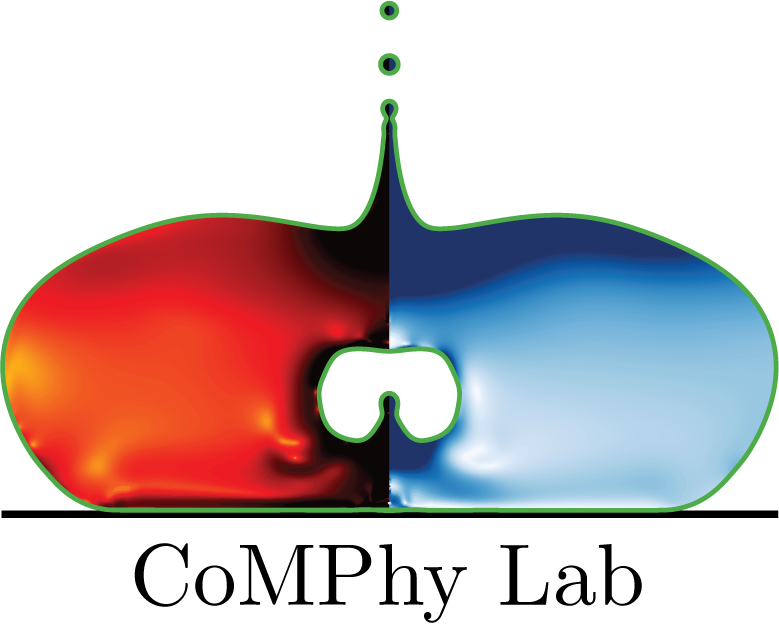
\includegraphics[height=2cm]{../_logosAndRef/CoMPhy-Lab.png}
\end{textblock*}

\vspace*{\headertobodysep}

\begin{center}
    \begin{LARGE}
     Pulling a Film from a Patchy Bath:\\ Langmuir--Blodgett Meets Landau--Levich
    \end{LARGE}
\end{center}

\noindent When a flat plate is withdrawn vertically from a quiescent bath, a thin liquid film is dragged out along with it. On a homogeneously wetting plate the thickness follows the Landau--Levich scaling $h \sim \ell_c \, \mathrm{Ca}^{2/3}$, where $\mathrm{Ca} = \eta U / \gamma$ compares viscous drag to capillary smoothing at the dynamic meniscus and $\ell_c = \sqrt{\gamma / (\rho g)}$ is the capillary length~\citep{landauLevich1942,quere1999fluid,rioBoulogne2017}. On a \emph{partially} wetting plate the story sharpens: below a critical capillary number $\mathrm{Ca}^\star$ set by dynamic wetting failure the contact line cannot keep up, and the plate emerges dry~\citep{bonnWettingSpreading2009}. That threshold is the throughput bottleneck of Langmuir--Blodgett deposition, the route by which lipid multilayers and membrane-protein arrays are built molecule by molecule on a substrate passing through a compressed monolayer. Pre-coat the plate with a patterned soft layer --- vesicle patches, protein prints, lithographic wettability stripes --- and the contact line pins on patches of characteristic size $\ell_p$. Pinning injects a new length scale into the meniscus problem. A second dimensionless group $\Lambda = \ell_p / (\ell_c \, \mathrm{Ca}^{1/3})$, comparing patch size to the dynamic-meniscus length, then decides whether the meniscus averages over many patches or resolves them one at a time. This MPhys or Master's-year project offers three parallel routes into the same question, and you pick the one that fits your strengths: analytical scaling, Basilisk~C simulation of the withdrawn film with spatial wettability, or the companion Langmuir--Blodgett experiment in Prof.~Bromley's laboratory (Durham Physics). The three routes answer the same question from different sides; a student takes only one.

\begin{tcolorbox}[colback=mgray,colframe=mpurple,title=TL;DR]
Three parallel routes to the same question, of which a student picks one: (i) derive the scaling theory of a coated Landau--Levich withdrawal, or (ii) build a Basilisk~C simulation of the same geometry with spatially varying wettability (with Dr~Vatsal~Sanjay, CoMPhy Lab), or (iii) run the companion Langmuir--Blodgett experiment on a patterned glass slide with designed proteins and lipid vesicles in a compressed amphiphile monolayer (with Prof.~Beth~Bromley, Durham Physics). One question runs through all three: how does a pre-existing patchy coating of size $\ell_p$ and areal fraction $\phi$ reshape the critical capillary number for film entrainment~\citep{bonnWettingSpreading2009}? The shared target is the $(\mathrm{Ca}, \Lambda)$ regime diagram with $\Lambda = \ell_p / (\ell_c \, \mathrm{Ca}^{1/3})$; theory, simulation, and experiment each anchor it from their own side.
\end{tcolorbox}

\section*{Description}

The classical derivation sits on a two-region matched asymptotic balance~\citep{landauLevich1942, quere1999fluid, rioBoulogne2017}. Far from the plate the meniscus is static, curved on the capillary length $\ell_c$. Close to the plate, a dynamic meniscus of length $\ell_m \sim \ell_c \, \mathrm{Ca}^{1/3}$ matches the static meniscus to the flat entrained film. Balancing viscous drag $\eta U / h^2$ against capillary smoothing $\gamma \partial_x^3 h$ in the dynamic meniscus fixes the thickness, $h \sim \ell_c \, \mathrm{Ca}^{2/3}$. On a completely wetting plate the contact line carries no additional stress and the derivation is closed. On a partially wetting plate the static contact angle $\theta_e$ sets an upper bound on how fast the three-phase line can advance before dynamic wetting failure forces transition to a Landau--Levich film, yielding a critical $\mathrm{Ca}^\star$ that depends sharply on $\theta_e$~\citep{eggers2004,snoeijerWetting2006,snoeijer2008,bonnWettingSpreading2009}. It is this partial-wetting threshold, not the pure Landau--Levich law, that caps the pull-out speed of Langmuir--Blodgett deposition.

In Prof.~Bromley's laboratory, a Langmuir trough holds a compressed amphiphile monolayer at the water surface, through which a substrate is withdrawn; proteins and lipid vesicles in the sub-phase adsorb onto the plate. The compression is held at a target surface pressure during deposition, and the transfer ratio fixes the deposited mass per dip. Four patterning routes give complementary handles on patch geometry: vesicle splatting leaves membrane patches of $\mathcal{O}(50\text{--}100)$\,nm; protein prints via dip-pen nanolithography leave engineered patches of $\mathcal{O}(10^2\text{--}10^3)$\,nm; micro-contact printing of mixed self-assembled monolayers~\citep{wilbur1994,mrksich1995} gives wettability-contrasted patches at $\mathcal{O}(1\text{--}10)$\,\micro m; and photolithographic wettability contrast~\citep{darhuber2000} gives stripes up to $\mathcal{O}(10\text{--}10^2)$\,\micro m. For Langmuir--Blodgett-relevant capillary numbers ($\mathrm{Ca} \sim 10^{-7}$--$10^{-4}$, so $\ell_m = \ell_c \, \mathrm{Ca}^{1/3}$ spans $\mathcal{O}(10\text{--}10^2)$\,\micro m), vesicle and dip-pen patches sit deep in the homogenised $\Lambda \ll 1$ regime; micro-contact-printed SAMs approach the $\Lambda \sim 1$ shoulder; photolithographic stripes push into $\Lambda \gtrsim 1$. The four routes together place $\ell_p$ across three decades and straddle the crossover in $\Lambda$.

The patchy plate introduces four substrate-side dimensionless controls beyond $\mathrm{Ca}$: the patch areal fraction $\phi$; the geometric ratio $\Lambda = \ell_p / \ell_m = \ell_p / (\ell_c \, \mathrm{Ca}^{1/3})$; the equilibrium contact-angle contrast $\Delta\theta = \theta_e^{\mathrm{wet}} - \theta_e^{\mathrm{dry}}$ between wettable and less-wettable patches; and the substrate hysteresis $\Delta\theta_{\mathrm{hyst}} = \theta_A - \theta_R$ between advancing and receding limits on a single patch. Where the patterning is anisotropic (stripes rather than spots), a fifth geometric control enters, $\chi = \ell_\parallel / \ell_\perp$, comparing patch lengths parallel and perpendicular to the pull-out direction. Two asymptotic limits follow. For $\Lambda \ll 1$ the dynamic meniscus integrates over many patches; the substrate acts homogenised with an effective contact angle $\theta_{\mathrm{eff}}(\phi, \Delta\theta)$ set by Cassie averaging, and the Landau--Levich prefactor shifts but the functional form is preserved~\citep{bonnWettingSpreading2009}. For $\Lambda \gtrsim 1$ the meniscus resolves individual patches and the contact line advances patch-by-patch; the defensible prediction is \emph{selective} deposition, with liquid preferentially transferred onto wettable regions rather than entrained as a uniform film~\citep{darhuber2000,maleki2007}. Whether a \emph{sub-critical} entrainment window (entrainment at $\mathrm{Ca} < \mathrm{Ca}^\star$) opens on the patchy substrate, and which of $\phi$, $\Delta\theta$, $\Delta\theta_{\mathrm{hyst}}$, $\chi$ governs any such threshold shift, is an open question this project is designed to settle.

Two further controls enter from the liquid side and the coating itself. If the pre-existing coating is an elastic film of thickness $t$ on a rigid substrate (a hydrated protein layer, a soft polymer stripe), substrate deformation at the contact line adds the thin-layer elastocapillary length $\ell_{ec} = \sqrt{t \gamma / E^\ast}$, with $E^\ast$ the reduced modulus of the layer~\citep{bertin2022}; the ratio $\ell_{ec}/\ell_p$ decides whether capillary forces deform individual patches. On the liquid side, the compressed amphiphile monolayer carries a surface elasticity $E_s = -A \, \partial \Pi / \partial A$, giving a Marangoni number $M_s = E_s / \gamma$ that modulates the dynamic meniscus independent of substrate physics; at typical deposition pressures ($\Pi \sim 30$\,mN/m for DPPC), $M_s$ reaches $\mathcal{O}(1)$ and must be carried explicitly in any scaling derivation. Mapping the full $(\mathrm{Ca}, \Lambda, \phi, \Delta\theta, \Delta\theta_{\mathrm{hyst}}, \chi, \ell_{ec}/\ell_p, M_s)$ response surface is out of reach for a single Master's-year project; locating the $\Lambda \sim 1$ crossover at fixed $(\phi, \Delta\theta)$ along one patterning route is the scientific target.

\begin{figure}[H]
    \begin{center}
        % TBD: schematic -- clean Landau--Levich meniscus (left) vs patchy substrate (right)
        % Suggested panels:
        %   (a) Homogeneous plate: static meniscus + dynamic meniscus matching region,
        %       film of thickness h = l_c Ca^{2/3}, labels for l_c, l_c Ca^{1/3}, h, U.
        %   (b) Patchy plate: contact line pinned on soft patches of size l_p;
        %       area fraction phi; patches shown smaller than, comparable to, and
        %       larger than the dynamic-meniscus length in three sub-panels so
        %       the Lambda < 1, Lambda ~ 1, Lambda > 1 regimes are visible.
        \fbox{\parbox{0.9\textwidth}{\centering \vspace{2cm} Figure~1 placeholder: \\ clean Landau--Levich meniscus vs pinning on a patchy coating \vspace{2cm}}}
        \caption{Clean-plate Landau--Levich vs the coated-plate hook. (a)~Homogeneous plate: the dynamic meniscus of length $\ell_m \sim \ell_c \, \mathrm{Ca}^{1/3}$ matches the static meniscus to a flat film of thickness $h \sim \ell_c \, \mathrm{Ca}^{2/3}$; on partially wetting substrates, $\mathrm{Ca} < \mathrm{Ca}^\star$ leaves the plate dry. (b)~Patchy plate: the contact line pins on patches of size $\ell_p$ and areal fraction $\phi$. The dimensionless group $\Lambda = \ell_p / \ell_m$ decides whether the dynamic meniscus averages over many patches ($\Lambda \ll 1$), resolves individual patches ($\Lambda \sim 1$), or advances fully patch-by-patch ($\Lambda \gg 1$).}
        \label{fig:mechanism}
    \end{center}
\end{figure}

The project offers three parallel routes onto that response surface, and a student picks one. The analytical route fixes the two asymptotic limits of the patchy Landau--Levich scaling, the dependence of the effective threshold on $\phi$ and the patch contact-angle contrast $\Delta\theta$, and the location of the $\Lambda \sim 1$ crossover. The computational route builds a two-dimensional Cartesian Basilisk~C simulation of the withdrawn film for transverse-stripe patterning, with spatial wettability imposed through the \texttt{contact.h} infrastructure~\citep{popinet2015quadtree,basiliskVatsal,basiliskVatsalDropFilm}; because \texttt{contact.h} sets only the geometric contact angle, the effective dynamic contact-angle response is calibrated against a partial-wetting benchmark in the spirit of~\citet{afkhami2009,afkhami2018} before any sweep, and the imposed $\theta_e(x)$ is smoothed over the three-to-five finest cells at patch edges to avoid mesh-locked spurious pinning. $(\mathrm{Ca}, \Lambda)$ is then swept at fixed $(\phi, \Delta\theta)$ to resolve the regime diagram; a disjoining-pressure closure for an elastic pre-coat~\citep{bertin2022} is a natural extension, not required for the Master's deliverable. The experimental route runs the companion Langmuir--Blodgett sweep in Prof.~Bromley's laboratory: compressed monolayer at fixed surface pressure, patterned substrate (vesicle splatting, dip-pen nanolithography of proteins, micro-contact-printed mixed self-assembled monolayers~\citep{wilbur1994,mrksich1995}, or photolithographic wettability contrast~\citep{darhuber2000}), and entrained-film thickness measured against pull-out speed across patch densities. Each route answers the same question from its own side.

The deliverable is a predictive rule. Given a target entrained-film thickness at a given pull-out speed, the regime diagram says which patch size, areal fraction, and contact-angle contrast deliver it --- and, where $\Lambda \gtrsim 1$, which patch geometry drives \emph{selective} deposition onto wettable regions rather than uniform entrainment. That rule matters because the Langmuir--Blodgett throughput bottleneck is the rate-limiting step for scaled manufacture of lipid-multilayer biosensors, membrane-protein arrays, and the functionalised surfaces of soft-electronic and soft-biomedical stacks. All simulation code, analysis scripts, and experimental data are released under the CoMPhy Lab open-source workflow on GitHub.

\begin{figure}[H]
    \begin{center}
        % TBD: (Ca, Lambda) regime diagram sketch with experimental + simulation markers
        % Suggested: log-log (Ca, Lambda) plane. Three regions:
        %   (i)  Lambda << 1: homogenised Landau--Levich with shifted prefactor.
        %   (ii) Lambda ~ O(1): resonant / crossover regime.
        %   (iii) Lambda >> 1: patch-by-patch entrainment; sub-critical window
        %         below the clean-plate Ca*.
        % Overlay: Basilisk DNS markers (colour-coded by phi) + LB experimental
        % points from the Bromley rig. Dashed line Ca* for clean plate.
        \fbox{\parbox{0.9\textwidth}{\centering \vspace{2cm} Figure~2 placeholder: \\ $(\mathrm{Ca}, \Lambda)$ regime diagram with LB experiment + Basilisk DNS markers \vspace{2cm}}}
        \caption{Target regime diagram on the $(\mathrm{Ca}, \Lambda)$ plane, with the clean-plate Landau--Levich threshold $\mathrm{Ca}^\star$ as the $\Lambda \to 0$ reference. Three regimes: homogenised ($\Lambda \ll 1$), resonant ($\Lambda \sim 1$), and isolated-patch entrainment ($\Lambda \gg 1$). Markers from Langmuir--Blodgett experiment (Bromley lab) and Basilisk~C axisymmetric simulation (CoMPhy Lab).}
        \label{fig:regime-map}
    \end{center}
\end{figure}

\section*{What you will do and what you will learn?}

\noindent The project has a shared foundation, three parallel routes (pick the one that fits your strengths), and a shared closure:

\begin{enumerate}
\itemsep0em
\item \textbf{Foundation.} Re-derive the classical Landau--Levich scaling $h \sim \ell_c \, \mathrm{Ca}^{2/3}$ from the matched-asymptotic balance at the dynamic meniscus~\citep{landauLevich1942,quere1999fluid}, and derive the partial-wetting critical capillary number $\mathrm{Ca}^\star(\theta_e)$ set by dynamic wetting failure~\citep{bonnWettingSpreading2009}.
\item \textbf{Analytical route.} Extend the derivation to a patchy substrate in two asymptotic limits: the homogenised limit $\Lambda = \ell_p / \ell_m \ll 1$ with a Cassie-averaged effective contact angle, and the patch-resolved limit $\Lambda \gtrsim 1$ with contact-line pinning patch-by-patch; locate the crossover analytically and fix the dependence on patch areal fraction $\phi$ and contact-angle contrast $\Delta\theta$.
\item \textbf{Computational route.} Build a two-dimensional Cartesian Basilisk~C simulation of the withdrawn film under transverse-stripe wettability via \texttt{contact.h}~\citep{popinet2015quadtree,basiliskVatsal,basiliskVatsalDropFilm}, calibrated against a partial-wetting benchmark in the spirit of~\citet{afkhami2009,afkhami2018} with $\theta_e(x)$ smoothed over the three-to-five finest cells at patch edges; sweep $(\mathrm{Ca}, \Lambda)$ at fixed $(\phi, \Delta\theta)$ to resolve the regime diagram. A disjoining-pressure closure for an elastic pre-coat~\citep{bertin2022} is a natural extension, not required for the Master's deliverable.
\item \textbf{Experimental route.} Run the companion Langmuir--Blodgett experiment in Prof.~Bromley's laboratory: compressed amphiphile monolayer on a Langmuir trough held at fixed surface pressure, patterned substrate (vesicle splatting, dip-pen nanolithography of proteins, micro-contact-printed mixed self-assembled monolayers~\citep{wilbur1994,mrksich1995}, or photolithographic wettability contrast~\citep{darhuber2000}), and entrained-film thickness measured against pull-out speed across patch densities.
\item \textbf{Closure.} Place your route's contribution on the $(\mathrm{Ca}, \Lambda)$ regime diagram, identify whether the $(\phi, \Lambda, \Delta\theta)$ window admits sub-critical entrainment or selective deposition onto wettable patches, and release all code, analysis scripts, and data under the CoMPhy Lab open-source workflow.
\end{enumerate}

\section*{Industrial and scientific context}

Langmuir--Blodgett deposition is the workhorse technique for assembling sub-monolayer to multi-layer films one molecule thick at a time~\citep{bonnWettingSpreading2009}; its canonical target in the Bromley laboratory is the functional supported membrane --- lipid bilayers and engineered membrane-protein arrays on glass or silicon. Throughput is capped by the partial-wetting critical capillary number $\mathrm{Ca}^\star$: too fast, and the contact line breaks down into dynamic wetting failure; too slow, and the per-dip rate collapses below what is useful for scaled manufacture. The clean-plate scaling is well understood~\citep{landauLevich1942,quere1999fluid,rioBoulogne2017}, but the substrate in a Langmuir--Blodgett transfer is \emph{never} clean: it carries the pre-existing patch structure deposited on the previous dip, and for biologically functional surfaces that structure is both heterogeneous and soft. No predictive continuum description covers the pre-coated regime, and no systematic experimental map of entrained-film thickness against patch geometry has been placed alongside one. Closing that gap --- analytically, numerically, and experimentally --- gives a design rule for sub-critical entrainment: given the patch areal fraction and contact-angle contrast produced by a chosen biological or lithographic patterning route, predict the pull-out speed that delivers a target multilayer thickness. The project sits squarely in the soft-matter / condensed-matter-physics interface: dynamic wetting of heterogeneous substrates~\citep{bonnWettingSpreading2009}, elastocapillary deformation of thin soft pre-coats~\citep{bertin2022}, and open-source multiphase CFD~\citep{popinet2015quadtree,basiliskVatsal}. For a Durham MPhys or Master's student, the project offers three complementary outputs, any one of which is a full Master's-year deliverable: the matched-asymptotic theory of the patchy threshold, the Basilisk~C simulation framework for heterogeneous-wettability dip-coating, or the first Langmuir--Blodgett dataset on heterogeneous substrates. Each anchors the $(\mathrm{Ca}, \Lambda)$ regime diagram from its own side.

If you have any questions, feel free to contact us \href{mailto:vatsal.sanjay@comphy-lab.org}{vatsal.sanjay@comphy-lab.org}/\\\href{mailto:vatsal.sanjay@durham.ac.uk}{vatsal.sanjay@durham.ac.uk} or drop by Ph255 (Rochester building) at the Department of Physics at Durham University.

\begin{center}
\begin{tabular}{|l|l|l|}
\hline \textbf{Collaborators} & \textbf{E-mail} & \textbf{Based at} \\
\hline \multirow{2}{*}{Dr. Vatsal Sanjay} & \href{mailto:vatsal.sanjay@comphy-lab.org}{vatsal.sanjay@comphy-lab.org} & \multirow{2}{*}{Ph255 (Rochester building)} \\
& \href{mailto:vatsal.sanjay@durham.ac.uk}{vatsal.sanjay@durham.ac.uk} & \\
\hline Prof. Beth Bromley & \href{mailto:beth.bromley@durham.ac.uk}{beth.bromley@durham.ac.uk} & Dept. of Physics, Durham \\
\hline
\end{tabular}
\end{center}

\vspace{1em}
\noindent\textit{Last updated: \today}

\printbibliography
\end{document}
